\chapter{Computer System Architecture}

\section{Introduction}

Computer System Architecture describes the organization and interaction of hardware components that execute programs and support operating systems. Understanding architecture is fundamental for operating systems because the OS directly manages processors, memory, devices, interrupts, and protection mechanisms.

From an interview perspective, computer architecture concepts frequently appear in discussions about processes, memory management, concurrency, virtualization, performance optimization, and system design.

\section{Computer System Overview}

A computer system consists of hardware and software working together to execute instructions and manage resources.

\subsection{Major Components}

\begin{itemize}
\item Central Processing Unit (CPU)
\item Main Memory (RAM)
\item Secondary Storage
\item Input Devices
\item Output Devices
\item System Bus
\item I/O Controllers
\item Operating System
\end{itemize}

\subsection{High-Level Architecture}

\begin{figure}[H]
\centering
\begin{tikzpicture}[node distance=2cm]

\node[draw, rectangle] (cpu) {CPU};
\node[draw, rectangle, right=3cm of cpu] (memory) {Main Memory};
\node[draw, rectangle, below=2cm of cpu] (io) {I/O Controllers};
\node[draw, rectangle, below=2cm of memory] (disk) {Storage};

\draw[<->] (cpu) -- node[above]{System Bus} (memory);
\draw[<->] (cpu) -- (io);
\draw[<->] (memory) -- (disk);
\draw[<->] (io) -- (disk);

\end{tikzpicture}
\caption{Basic Computer System Architecture}
\end{figure}

\subsection{Von Neumann Architecture}

Most modern systems follow the Von Neumann model.

Characteristics:

\begin{itemize}
\item Shared memory for instructions and data
\item Sequential instruction execution
\item Program stored in memory
\item CPU fetches instructions from memory
\end{itemize}

\section{CPU Architecture}

The CPU executes instructions and coordinates system activities.

\subsection{CPU Components}

\begin{itemize}
\item Arithmetic Logic Unit (ALU)
\item Control Unit
\item Registers
\item Cache
\item Instruction Decoder
\item Execution Units
\end{itemize}

\begin{figure}[H]
\centering
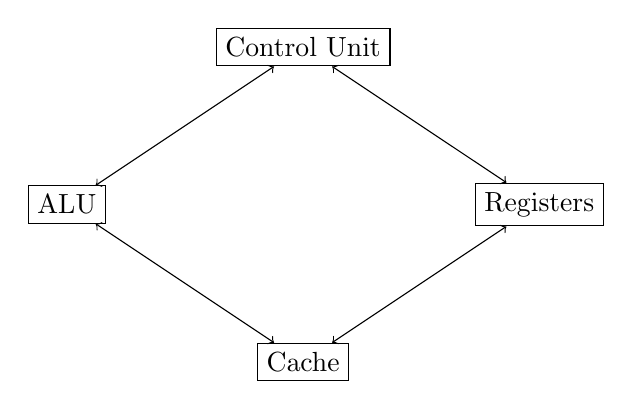
\begin{tikzpicture}

\node[draw, rectangle] (control) at (0,2) {Control Unit};

\node[draw, rectangle] (alu) at (-3,0) {ALU};

\node[draw, rectangle] (reg) at (3,0) {Registers};

\node[draw, rectangle] (cache) at (0,-2) {Cache};

\draw[<->] (control) -- (alu);
\draw[<->] (control) -- (reg);
\draw[<->] (alu) -- (cache);
\draw[<->] (reg) -- (cache);

\end{tikzpicture}
\caption{CPU Internal Organization}
\end{figure}

\section{Registers}

Registers are the fastest storage locations in a computer.

\subsection{Characteristics}

\begin{itemize}
\item Located inside CPU
\item Very low access latency
\item Hold frequently used data
\item Limited quantity
\end{itemize}

\subsection{Common Registers}

\begin{longtable}{|p{4cm}|p{9cm}|}
\hline
Register & Purpose \
\hline
General Purpose Registers & Store operands and intermediate results \
\hline
Program Counter & Address of next instruction \
\hline
Stack Pointer & Points to stack top \
\hline
Instruction Register & Current instruction \
\hline
Status Register & Condition flags \
\hline
Base Register & Memory relocation \
\hline
Index Register & Address calculation \
\hline
\end{longtable}

\section{Program Counter}

Program Counter (PC) stores the address of the next instruction to execute.

\subsection{Operation}

\begin{enumerate}
\item Fetch instruction from PC address
\item Execute instruction
\item Increment PC
\item Update PC for branch instructions
\end{enumerate}

\subsection{Example}

\begin{center}
PC = 1000
\end{center}

Instruction at 1000 executes.

PC becomes:

\begin{center}
1004
\end{center}

assuming instruction length is 4 bytes.

\section{Stack Pointer}

Stack Pointer (SP) points to the top of the stack.

\subsection{Uses}

\begin{itemize}
\item Function calls
\item Local variables
\item Return addresses
\item Context switching
\item Interrupt handling
\end{itemize}

\subsection{Stack Layout}

\begin{figure}[H]
\centering
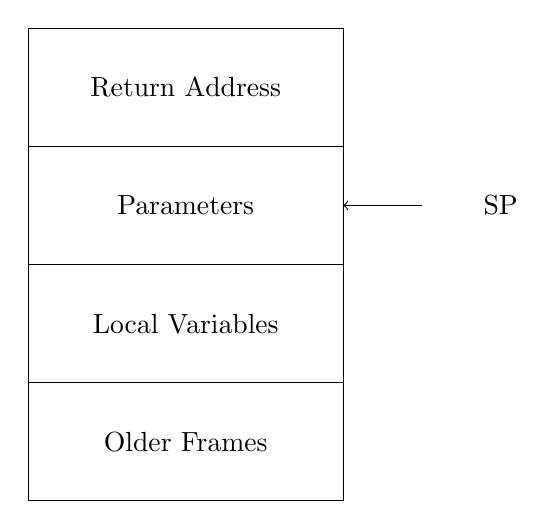
\begin{tikzpicture}

\draw (0,0) rectangle (4,6);

\draw (0,1.5) -- (4,1.5);
\draw (0,3) -- (4,3);
\draw (0,4.5) -- (4,4.5);

\node at (2,5.25) {Return Address};
\node at (2,3.75) {Parameters};
\node at (2,2.25) {Local Variables};
\node at (2,0.75) {Older Frames};

\draw[->] (5,3.75) -- (4,3.75);
\node at (6,3.75) {SP};

\end{tikzpicture}
\caption{Stack Structure}
\end{figure}

\section{Memory Hierarchy}

Memory hierarchy balances cost, speed, and capacity.

\subsection{Hierarchy Levels}

\begin{figure}[H]
\centering
\begin{tikzpicture}

\node[draw,trapezium,trapezium left angle=70,trapezium right angle=110] (r) at (0,6) {Registers};

\node[draw,trapezium,trapezium left angle=70,trapezium right angle=110] (l1) at (0,4.5) {L1 Cache};

\node[draw,trapezium,trapezium left angle=70,trapezium right angle=110] (l2) at (0,3) {L2 Cache};

\node[draw,trapezium,trapezium left angle=70,trapezium right angle=110] (ram) at (0,1.5) {RAM};

\node[draw,trapezium,trapezium left angle=70,trapezium right angle=110] (disk) at (0,0) {SSD/HDD};

\end{tikzpicture}
\caption{Memory Hierarchy}
\end{figure}

\subsection{Hierarchy Comparison}

\begin{longtable}{|p{3cm}|p{3cm}|p{3cm}|p{3cm}|}
\hline
Level & Speed & Cost & Capacity \
\hline
Registers & Highest & Highest & Lowest \
\hline
L1 Cache & Very High & High & Small \
\hline
L2 Cache & High & Medium & Moderate \
\hline
RAM & Moderate & Lower & Large \
\hline
Disk & Slow & Lowest & Very Large \
\hline
\end{longtable}

\section{Instruction Cycle}

Instruction cycle is the sequence of operations required to execute an instruction.

Stages:

\begin{enumerate}
\item Fetch
\item Decode
\item Execute
\item Memory Access
\item Write Back
\end{enumerate}

\section{Fetch Decode Execute Cycle}

\begin{figure}[H]
\centering
\begin{tikzpicture}[node distance=3cm]

\node[draw, rectangle] (fetch) {Fetch};

\node[draw, rectangle, right=of fetch] (decode) {Decode};

\node[draw, rectangle, right=of decode] (execute) {Execute};

\draw[->] (fetch) -- (decode);
\draw[->] (decode) -- (execute);
\draw[->] (execute) .. controls +(0,-1) and +(0,-1) .. (fetch);

\end{tikzpicture}
\caption{Fetch Decode Execute Cycle}
\end{figure}

\subsection{Fetch}

CPU retrieves instruction from memory.

\subsection{Decode}

Instruction decoder interprets operation.

\subsection{Execute}

ALU or execution units perform requested task.

\section{Interrupts}

Interrupts notify CPU about events requiring immediate attention.

\subsection{Types}

\begin{itemize}
\item Hardware Interrupts
\item Software Interrupts
\item Maskable Interrupts
\item Non-Maskable Interrupts
\end{itemize}

\subsection{Interrupt Handling Flow}

\begin{enumerate}
\item Device generates interrupt
\item CPU saves context
\item Interrupt vector lookup
\item ISR executes
\item Context restored
\item Resume execution
\end{enumerate}

\begin{figure}[H]
\centering
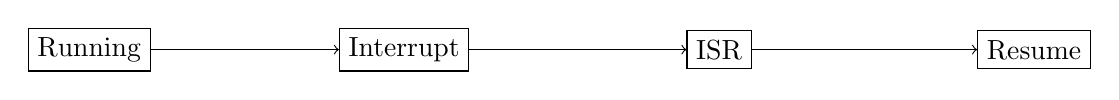
\begin{tikzpicture}

\node[draw] (run) at (0,0) {Running};

\node[draw] (int) at (4,0) {Interrupt};

\node[draw] (isr) at (8,0) {ISR};

\node[draw] (resume) at (12,0) {Resume};

\draw[->] (run) -- (int);
\draw[->] (int) -- (isr);
\draw[->] (isr) -- (resume);

\end{tikzpicture}
\caption{Interrupt Processing}
\end{figure}

\section{Trap Handling}

A trap is a software-generated interrupt.

\subsection{Examples}

\begin{itemize}
\item System calls
\item Breakpoints
\item Debugging operations
\end{itemize}

\subsection{Flow}

\begin{enumerate}
\item User process issues trap
\item CPU switches to kernel mode
\item Kernel executes service
\item Return to user mode
\end{enumerate}

\section{Exceptions}

Exceptions are unexpected conditions occurring during instruction execution.

\subsection{Examples}

\begin{itemize}
\item Divide by zero
\item Invalid opcode
\item Page fault
\item Arithmetic overflow
\end{itemize}

\subsection{Classification}

\begin{longtable}{|p{3cm}|p{9cm}|}
\hline
Type & Description \
\hline
Fault & Recoverable exception \
\hline
Trap & Intentional exception \
\hline
Abort & Severe unrecoverable error \
\hline
\end{longtable}

\section{DMA}

Direct Memory Access allows devices to transfer data directly to memory without CPU involvement.

\subsection{Advantages}

\begin{itemize}
\item Reduces CPU overhead
\item Improves throughput
\item Enables parallelism
\end{itemize}

\subsection{DMA Operation}

\begin{figure}[H]
\centering
\begin{tikzpicture}

\node[draw] (cpu) at (0,0) {CPU};
\node[draw] (dma) at (4,0) {DMA Controller};
\node[draw] (ram) at (8,0) {RAM};
\node[draw] (disk) at (4,-3) {Disk};

\draw[->] (cpu) -- (dma);
\draw[<->] (dma) -- (ram);
\draw[<->] (dma) -- (disk);

\end{tikzpicture}
\caption{DMA Data Transfer}
\end{figure}

\section{Cache Memory}

Cache memory reduces average memory access time.

\subsection{Why Cache Works}

Based on locality principles:

\begin{itemize}
\item Temporal Locality
\item Spatial Locality
\end{itemize}

\subsection{Cache Levels}

\begin{itemize}
\item L1 Cache
\item L2 Cache
\item L3 Cache
\end{itemize}

\subsection{Cache Metrics}

[
\text{Hit Ratio}
================

\frac{\text{Cache Hits}}
{\text{Total Accesses}}
]

\subsection{Interview Insight}

A cache hit is significantly faster than a cache miss because the CPU avoids accessing slower memory.

\section{Multicore Systems}

Modern CPUs contain multiple processing cores.

\subsection{Benefits}

\begin{itemize}
\item Parallel execution
\item Better throughput
\item Improved responsiveness
\item Efficient multitasking
\end{itemize}

\subsection{Architecture}

\begin{figure}[H]
\centering
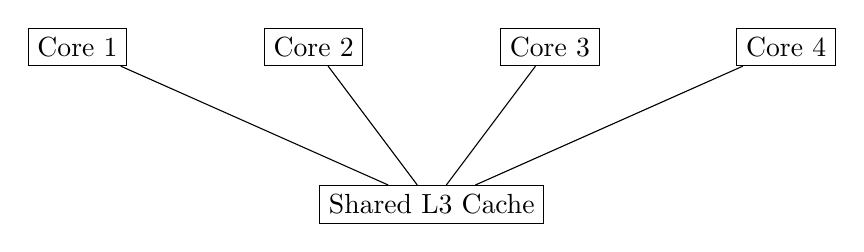
\begin{tikzpicture}

\node[draw] (c1) at (0,0) {Core 1};
\node[draw] (c2) at (3,0) {Core 2};
\node[draw] (c3) at (6,0) {Core 3};
\node[draw] (c4) at (9,0) {Core 4};

\node[draw] (cache) at (4.5,-2) {Shared L3 Cache};

\draw (c1)--(cache);
\draw (c2)--(cache);
\draw (c3)--(cache);
\draw (c4)--(cache);

\end{tikzpicture}
\caption{Multicore Processor}
\end{figure}

\section{NUMA Architecture}

NUMA stands for Non-Uniform Memory Access.

\subsection{Concept}

Memory access time depends on memory location relative to processor.

\subsection{Architecture}

\begin{figure}[H]
\centering
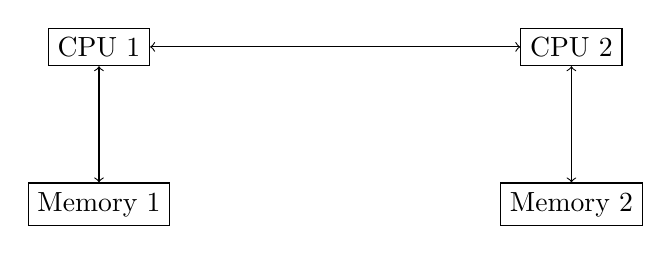
\begin{tikzpicture}

\node[draw] (cpu1) at (0,0) {CPU 1};
\node[draw] (mem1) at (0,-2) {Memory 1};

\node[draw] (cpu2) at (6,0) {CPU 2};
\node[draw] (mem2) at (6,-2) {Memory 2};

\draw[<->] (cpu1) -- (mem1);
\draw[<->] (cpu2) -- (mem2);
\draw[<->] (cpu1) -- (cpu2);

\end{tikzpicture}
\caption{NUMA Organization}
\end{figure}

\subsection{Characteristics}

\begin{itemize}
\item Local memory access is faster
\item Remote memory access is slower
\item Common in large servers
\end{itemize}

\section{Hardware Protection Mechanisms}

Protection mechanisms prevent unauthorized access.

\subsection{Goals}

\begin{itemize}
\item Isolation
\item Security
\item Reliability
\item Resource control
\end{itemize}

\subsection{Mechanisms}

\begin{itemize}
\item Memory Protection
\item Privilege Levels
\item MMU
\item Access Control Bits
\item Segmentation
\item Paging
\end{itemize}

\section{User Mode and Privileged Instructions}

Modern processors support multiple execution modes.

\subsection{User Mode}

\begin{itemize}
\item Restricted access
\item Application execution
\item Cannot execute privileged instructions
\end{itemize}

\subsection{Kernel Mode}

\begin{itemize}
\item Full hardware access
\item Executes operating system code
\item Handles interrupts and exceptions
\end{itemize}

\subsection{Privileged Instructions}

Examples:

\begin{itemize}
\item Modify page tables
\item Disable interrupts
\item Access device registers
\item Change processor mode
\end{itemize}

\subsection{Mode Transition}

\begin{figure}[H]
\centering
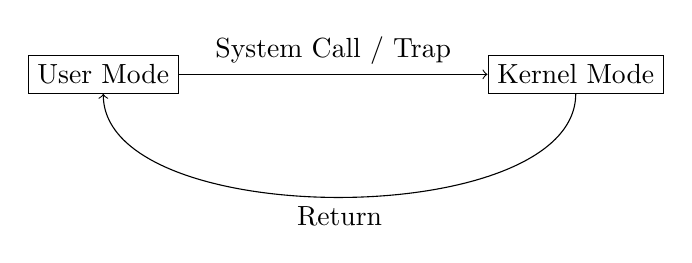
\begin{tikzpicture}

\node[draw] (user) at (0,0) {User Mode};

\node[draw] (kernel) at (6,0) {Kernel Mode};

\draw[->] (user) -- node[above]{System Call / Trap} (kernel);

\draw[->] (kernel) .. controls +(0,-2) and +(0,-2) .. node[below]{Return} (user);

\end{tikzpicture}
\caption{Mode Switching}
\end{figure}

\section{Interview Explanations}

\subsection{Why Are Registers Faster Than RAM?}

Registers reside inside the CPU and can be accessed without traversing memory buses.

\subsection{Why Are Interrupts Important?}

Without interrupts, CPUs would continuously poll devices, wasting processing cycles.

\subsection{Why Is Cache Needed?}

Processor speeds have increased much faster than memory speeds. Cache bridges this gap.

\subsection{Difference Between Interrupt and Trap}

Interrupts are usually external events while traps are software-generated.

\subsection{Why Does NUMA Exist?}

NUMA improves scalability in multiprocessor systems by distributing memory closer to processors.

\section{Key Takeaways}

\begin{keytakeaways}
Computer architecture forms the foundation of operating systems. CPUs execute instructions through the fetch-decode-execute cycle. Registers provide the fastest storage. Program Counter tracks instruction execution while Stack Pointer manages function calls. Memory hierarchy balances performance and cost. Interrupts, traps, and exceptions allow event-driven execution. DMA improves I/O efficiency. Cache memory exploits locality. Multicore and NUMA architectures enable scalability. Hardware protection mechanisms enforce security and isolation. User mode and kernel mode provide controlled hardware access.
\end{keytakeaways}

\section{Interview Questions with Answers}

\begin{enumerate}
\item \textbf{What is the Program Counter?}\
It stores the address of the next instruction to execute.

\item \textbf{What is the Stack Pointer?}\
It points to the current top of the stack.

\item \textbf{Why are registers faster than RAM?}\
Registers are located inside the CPU.

\item \textbf{What is cache memory?}\
High-speed memory storing frequently accessed data.

\item \textbf{What is temporal locality?}\
Recently used data is likely to be used again.

\item \textbf{What is spatial locality?}\
Nearby memory locations are likely to be accessed.

\item \textbf{What is DMA?}\
Direct transfer between devices and memory without CPU involvement.

\item \textbf{What is an interrupt?}\
A signal requiring CPU attention.

\item \textbf{What is a trap?}\
A software-generated interrupt.

\item \textbf{What is an exception?}\
An abnormal condition during instruction execution.

\item \textbf{What is NUMA?}\
Non-Uniform Memory Access architecture.

\item \textbf{Difference between user mode and kernel mode?}\
Kernel mode has unrestricted hardware access.

\item \textbf{Why are privileged instructions restricted?}\
To maintain system security and stability.

\item \textbf{What is a cache hit?}\
Requested data found in cache.

\item \textbf{What is a cache miss?}\
Requested data not found in cache.
\end{enumerate}

\section{MCQs with Answers}

\begin{enumerate}
\item CPU executes instructions using:
\begin{enumerate}[label=(\alph*)]
\item Paging
\item Scheduling
\item Fetch Decode Execute
\item Swapping
\end{enumerate}
Answer: (c)

\item Fastest memory is:
\begin{enumerate}[label=(\alph*)]
\item SSD
\item RAM
\item Cache
\item Registers
\end{enumerate}
Answer: (d)

\item PC stands for:
\begin{enumerate}[label=(\alph*)]
\item Program Counter
\item Process Controller
\item Page Counter
\item Priority Counter
\end{enumerate}
Answer: (a)

\item Stack Pointer points to:
\begin{enumerate}[label=(\alph*)]
\item Heap
\item Cache
\item Stack Top
\item Code Segment
\end{enumerate}
Answer: (c)

\item DMA reduces:
\begin{enumerate}[label=(\alph*)]
\item CPU Overhead
\item RAM
\item Disk Space
\item Threads
\end{enumerate}
Answer: (a)

\item NUMA stands for Non:
\begin{enumerate}[label=(\alph*)]
\item Unified
\item Uniform
\item Uniformed
\item Utility
\end{enumerate}
Answer: (b)

\item Cache exploits:
\begin{enumerate}[label=(\alph*)]
\item Locality
\item Fragmentation
\item Scheduling
\item Deadlock
\end{enumerate}
Answer: (a)

\item Interrupts are:
\begin{enumerate}[label=(\alph*)]
\item Events requiring attention
\item Files
\item Registers
\item Drivers
\end{enumerate}
Answer: (a)

\item Trap is:
\begin{enumerate}[label=(\alph*)]
\item Hardware interrupt
\item Software interrupt
\item Cache miss
\item DMA request
\end{enumerate}
Answer: (b)

\item User mode:
\begin{enumerate}[label=(\alph*)]
\item Full access
\item Restricted access
\item BIOS mode
\item DMA mode
\end{enumerate}
Answer: (b)

\item L1 cache is:
\begin{enumerate}[label=(\alph*)]
\item Slowest
\item Fastest cache
\item Disk cache
\item Network cache
\end{enumerate}
Answer: (b)

\item Exception example:
\begin{enumerate}[label=(\alph*)]
\item Divide by zero
\item Keyboard input
\item DMA transfer
\item Booting
\end{enumerate}
Answer: (a)

\item Multicore processors improve:
\begin{enumerate}[label=(\alph*)]
\item Parallelism
\item Fragmentation
\item Paging
\item Swapping
\end{enumerate}
Answer: (a)

\item Kernel mode can:
\begin{enumerate}[label=(\alph*)]
\item Execute privileged instructions
\item Access only RAM
\item Disable cache
\item None
\end{enumerate}
Answer: (a)

\item Memory hierarchy balances:
\begin{enumerate}[label=(\alph*)]
\item Speed and Cost
\item Threads and CPU
\item Interrupts and DMA
\item Files and Processes
\end{enumerate}
Answer: (a)
\end{enumerate}

\section{Revision Notes}

\begin{revisionnotes}
\item Registers are the fastest storage locations.
\item Program Counter stores next instruction address.
\item Stack Pointer tracks stack top.
\item CPU follows fetch-decode-execute cycle.
\item Interrupts are asynchronous events.
\item Traps are software-generated interrupts.
\item Exceptions occur during instruction execution.
\item DMA bypasses CPU during data transfer.
\item Cache reduces memory latency.
\item Locality principle enables effective caching.
\item Multicore CPUs improve parallel processing.
\item NUMA introduces local and remote memory access.
\item Hardware protection provides isolation.
\item User mode restricts hardware access.
\item Kernel mode executes privileged operations.
\end{revisionnotes}

\section{Cheat Sheet}

\begin{longtable}{|p{5cm}|p{8cm}|}
\hline
Concept & Summary \
\hline
CPU & Executes instructions \
\hline
Register & Fastest storage \
\hline
Program Counter & Next instruction address \
\hline
Stack Pointer & Stack top location \
\hline
Cache & High-speed memory \
\hline
L1 Cache & Fastest cache level \
\hline
DMA & Device-memory transfer without CPU \
\hline
Interrupt & External event notification \
\hline
Trap & Software interrupt \
\hline
Exception & Error during execution \
\hline
NUMA & Non-uniform memory access \
\hline
User Mode & Restricted execution \
\hline
Kernel Mode & Privileged execution \
\hline
Privileged Instruction & OS-only instruction \
\hline
Memory Hierarchy & Registers $\rightarrow$ Cache $\rightarrow$ RAM $\rightarrow$ Disk \
\hline
\end{longtable}
